\chapter{系统调用与fork}

\section{实验目的}
  \begin{enumerate}
    \item 掌握系统调用的概念及流程
    \item 实现进程间通讯机制
    \item 实现fork函数
  \end{enumerate}

在系统中真正被所有进程都使用的内核通信方式是系统调用,例如当进程请求内核服务时,就使用的是系统调用。
一般情况下,进程是不能够存取系统内核的,它不能存取内核使用的内存段,也不能调用内核函数,
CPU的硬件结构保证了这一点,只有系统调用是一个例外。
进程使用寄存器中适当的值跳转到内核中事先定义好的代码中执行(当然,这些代码是只读的)。
在这一节的实验中,我们需要实现系统调用机制,并再此基础上实现进程间通信(ipc)机制和fork。

\section{系统调用(System Call)}
本节中,我们着重讨论系统调用的作用,并完成实现相关的内容。

\subsection{一探到底,系统调用的来龙去脉}
说起系统调用,你冒出的第一个问题一定是:系统调用到底长什么样子?为了一探究竟,我们选择一个极为简单的程序作为实验对象。
在这个程序中,我们通过puts来输出一个字符串到终端。

\begin{minted}[linenos]{c}
#include <stdio.h>

int main() {
        puts("Hello World!\n");
        return 0;
}
\end{minted}

\begin{note}
如果你还记得C语言课上关于标准输出的相关知识的话,你一定知道在C语言中,终端被抽象为了标准输出文件stdout。
通过向标准输出文件写东西,就可以输出内容到屏幕。而向文件写入内容是通过write系统调用完成的。
因此,我们选择通过观察puts函数,来探究系统调用的奥秘。
\end{note}

我们通过GDB进行单步调试,逐步深入到函数之中,观察puts具体的调用过程\footnote{这里为了方便大家在自己的机器上重现,
我们选用了Linux X86\_64平台作为实验平台}。运行GDB,将断点设置在puts这条语句上,并通过stepi指令\footnote{为了加快调试进程,
可以尝试stepi N指令,N的位置填写任意数字均可。这样每次会执行N条机器指令。笔者使用的是stepi 10。}
单步进入到函数中。当程序到达write函数时停下,因为write正是Linux的一条系统调用。我们打印出此时的函数调用栈,
可以看出,C标准库中的puts函数实际上通过了很多层函数调用,最终调用到了底层的write函数进行真正的屏幕打印操作。

\begin{minted}[linenos]{objdump}
(gdb)
0x00007ffff7b1b4e0 in write () from /lib64/libc.so.6
(gdb) backtrace
#0  0x00007ffff7b1b4e0 in write () from /lib64/libc.so.6
#1  0x00007ffff7ab340f in _IO_file_write () from /lib64/libc.so.6
#2  0x00007ffff7ab2aa3 in ?? () from /lib64/libc.so.6
#3  0x00007ffff7ab4299 in _IO_do_write () from /lib64/libc.so.6
#4  0x00007ffff7ab462b in _IO_file_overflow () from /lib64/libc.so.6
#5  0x00007ffff7ab5361 in _IO_default_xsputn () from /lib64/libc.so.6
#6  0x00007ffff7ab3992 in _IO_file_xsputn () from /lib64/libc.so.6
#7  0x00007ffff7aaa4ef in puts () from /lib64/libc.so.6
#8  0x0000000000400564 in main () at test.c:4
\end{minted}

通过gdb显示的信息,我们可以看到,这个write()函数是在libc.so这个动态链接库中的,也就是说,它仍然是C库中的函数,
而不是内核中的函数。因此,该write()函数依旧是个用户空间函数。为了彻底揭开这个函数的秘密,我们对其进行反汇编。

\begin{minted}[linenos]{objdump}
(gdb) disassemble 0x00007ffff7b1b4e0
Dump of assembler code for function write:
=> 0x00007ffff7b1b4e0 <+0>:     cmpl   $0x0,0x2bf759(%rip)        # 0x7ffff7ddac40
   0x00007ffff7b1b4e7 <+7>:     jne    0x7ffff7b1b4f9 <write+25>
   0x00007ffff7b1b4e9 <+9>:     mov    $0x1,%eax
   0x00007ffff7b1b4ee <+14>:    syscall
   0x00007ffff7b1b4f0 <+16>:    cmp    \$0xfffffffffffff001,%rax
   0x00007ffff7b1b4f6 <+22>:    jae    0x7ffff7b1b529 <write+73>
   0x00007ffff7b1b4f8 <+24>:    retq
End of assembler dump.
\end{minted}

通过gdb的反汇编功能,我们可以看到,这个函数最终执行了syscall这个极为特殊的指令。从它的名字我们就能够猜出它的用途,
它使得进程陷入到内核态中,执行内核中的相应函数,完成相应的功能。在系统调用返回后,用户空间的相关函数会将系统调用的结果,
通过一系列的过程,最终返回给用户程序。

由此我们可以看到,系统调用实际上是操作系统和用户空间的一组接口。用户空间的程序通过系统调用来访问操作系统的一些服务,
谋求操作系统提供必要的帮助。

在进行了上面的一系列探究后,我们将我们的发现罗列出来,整理一下我们的思路:
\begin{itemize}
  \item 存在一些只能由操作系统来完成的操作(如读写设备、创建进程等)。
  \item 用户程序要实现一些功能(比如执行另一个程序、读写文件),必须依赖操作系统的帮助。
  \item C标准库中的一些函数的实现必须依赖于操作系统(如我们所探究的puts函数)。
  \item 通过执行syscall指令,我们可以陷入到内核态,请求操作系统的一些服务。
  \item 直接使用操作系统的功能是很繁复的(每次都需要设置必要的寄存器,并执行syscall指令)
\end{itemize}

之后,我们再来整理一下调用C标准库中的puts函数的过程中发生了什么:
\begin{enumerate}
  \item 调用puts函数
  \item 在一系列的函数调用后,最终调用了write函数。
  \item write函数设置了为寄存器设置了相应的值,并执行了syscall指令。
  \item 进入内核态,内核中相应的函数或服务被执行。
  \item 回到用户态的write函数中,将系统调用的结果从相关的寄存器中取回,并返回。
  \item 再次经过一系列的返回过程后,回到了puts函数中。
  \item puts函数返回。
\end{enumerate}

综合上面这些内容,相信你一定已经发现了其中的巧妙之处。操作系统将自己所能够提供的服务以系统调用的方式提供给用户空间。
用户程序即可通过操作系统来完成一些特殊的操作。同时,所有的特殊操作就全部在操作系统的掌控之中了
(因为用户程序只能通过由操作系统提供的系统调用来完成这些操作,所以操作系统可以确保用户不破坏系统的稳定)。
而直接使用这些系统调用较为麻烦,于是由产生了用户空间的一系列API,如POSIX、C标准库等,它们在系统调用的基础上,
实现更多更高级的常用功能,使得用户在编写程序时不用再处理这些繁琐而复杂的底层操作,
而是直接通过调用高层次的API就能实现各种功能。通过这样巧妙的层次划分,使得程序更为灵活,也具有了更好的可移植性。
对于用户程序来说,只要自己所依赖的API不变,无论底层的系统调用如何变化,都不会对自己造成影响,
使得程序更易于在不同的系统间移植。整个结构如图\ref{fig:api-and-syscall}所示。

\begin{figure}[htbp]
  \centering
  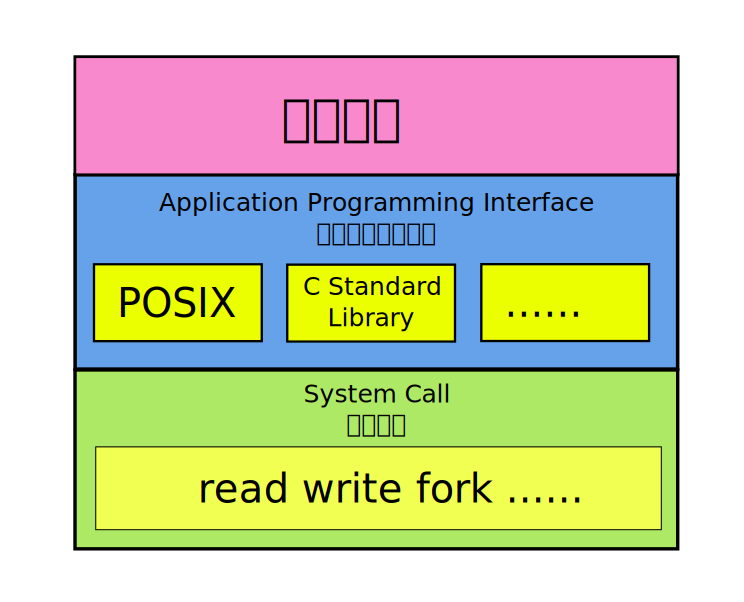
\includegraphics[width=7cm]{api-and-syscall}
  \caption{API、系统调用层次结构}\label{fig:api-and-syscall}
\end{figure}

\subsection{系统调用机制的实现}
在发现了系统调用的本质之后,我们就要着手在我们的小操作系统中实现一套系统调用机制了。不过,不要着急,为了使得后面的思路更清晰,
我们先来整理一下系统调用的流程:
\begin{enumerate}
  \item 调用库函数
  \item 调用一个用户空间的系统调用函数(用于封装设置寄存器、传参等繁复的操作)。
  \item 内核空间系统调用函数被执行。
  \item 从相应寄存器中收集返回值,并返回到库函数中。
  \item 库函数返回,回到用户程序
\end{enumerate}

也就是说,为了实现系统调用机制并实现我们自己的系统调用,我们需要找到内核空间中的系统调用函数,以及对应的用户空间系统调用函数。
不难发现,内核空间的系统调用实现在lib/syscall\_all.c中。在这段代码中,有大量的以sys开头的函数,这些函数便是内核空间的
系统调用的实现。

之后,我们再看用户空间的user/syscall\_lib.c,发现了一堆以syscall开头的函数,每个函数都根据传入的参数,调用了msyscall函数。
看到这里,你想到了什么?msyscall中一定是实际执行设置寄存器、执行syscall指令一类的底层操作的函数。
我们看到的这些syscall开头的函数为用户封装了这些繁复的过程。

这些syscall函数已经被预先实现好了,我们来看看msyscall函数。这个函数位于user/syscall\_wrap.S。
msyscall需要实现将必要的参数压栈,并执行syscall指令陷入内核态。

\begin{exercise}
填写msyscall,使得系统调用机制可以正常工作。
\end{exercise}

看到这个exercise你是不是觉得有些无语?完全没有可以参考的信息啊!我们从何知道这个msyscall如何填写呢?
仔细思考一下,msyscall的主要工作是设置栈、寄存器等,为后面的系统调用设置好参数。也就是说,想知道msyscall需要做些什么,
我们只需看一下后面内核中的相关代码是如何使用这些参数的就OK了。知道了内核用了什么,自然也就知道我们应当设置些什么。
内核处理系统调用的中断处理程序位于lib/syscall.S中,相应的注释已经预先加在了代码中,如代码\ref{code:handlesys.S}所示。

\begin{codeBoxWithCaption}{系统调用服务程序\label{code:handlesys.S}}
  \inputminted[linenos]{gas}{codes/handlesys.S}
\end{codeBoxWithCaption}

通过上面的代码,我们可以知道,所有的参数都应当按照顺序放入栈中。根据MIPS的ABI标准,前4个参数通过a0-a3寄存器传递,
后面的参数通过栈了传递。值得注意的是,标准要求程序必须分配足够容纳\textbf{所有}参数的栈空间。也就是说,尽管在函数调用的过程中,
前四个参数是通过寄存器来传递的,但程序依旧需要为其分配栈空间。也就是说,
GCC在生成调用msyscall函数的代码时已经按照标准为我们开了一个足够大的栈,我们在msyscall中只需将前四个参数压入到栈中即可,
无需再自行分配栈空间。

完成msyscall函数后,我们的小内核的系统调用机制便可以正常工作了。

\subsection{基础系统调用函数}

在系统调用机制搞定之后,我们自然是要弄几个系统调用玩一玩了。我们实现些什么系统调用呢?打开 lib/syscall\_all.c,可以看到玲琅满目的系统调用函数等着我们去填写。这些系统调用都是基础的系统调用,不论是之后的IPC还是fork,都需要这些基础的系统调用作为支撑。
首先我们看向sys\_mem\_alloc。这个函数的主要功能是分配内存,简单的说,用户程序可以通过这个系统调用给该程序所允许的虚拟内存空间内存分配实际的物理内存,需要用到一些我们之前在pmap.c中所定义的函数
\begin{exercise}
实现lib/syscall\_all.c中的int sys\_mem\_alloc(int sysno,u\_int envid, u\_int va, u\_int perm)函数
\end{exercise}
我们再来看sys\_mem\_map,这个函数的参数很多,但是意义也很直接:将源进程地址空间中的相应内存映射到目标进程的相应地址空间的相应虚拟内存中去。换句话说,此时两者共享着一页物理内存。
\begin{exercise}
实现lib/syscall\_all.c中的int sys\_mem\_map(int sysno,u\_int srcid, u\_int srcva, u\_int dstid, u\_dstva, u\_int perm)函数
\end{exercise}
关于内存的还有一个函数:sys\_mem\_unmap, 正如字面意义所显示的,这个系统调用的功能是解除某个进程地址空间虚拟内存和物理内存之间的映射关系。
\begin{exercise}
实现lib/syscall\_all.c中的int sys\_mem\_unmap(int sysno,u\_int envid, u\_int va)函数
\end{exercise}
除了与内存相关的函数外,另外一个常用的系统调用函数是sys\_yield,这个函数的功能主要就在于实现用户进程对CPU的放弃,可以利用我们之前已经编写好的函数,
另外为了通过我们之前编写的进程切换机制保存现场,这里需要在KERNEL\_SP和TIMESTACK上做一点准备工作
\begin{exercise}
实现lib/syscall\_all.c中的void sys\_yield(void)函数
\end{exercise}
可能你也注意到了,在此我们的系统调用函数并没使用到它的第一个参数sysno,在这里,sysno作为系统调用号被传入,现在起的更多是一个”占位“的作用,能和之前用户层面的系统调用函数参数顺序相匹配,更好理解。
\section{进程间通信机制(Inter-Process Communication)}
在系统调用机制搞定之后,我们自然是要弄几个系统调用玩一玩了。作为一个微内核系统,我们要来实现个什么系统调用呢?
没错,当然是IPC了。IPC可是微内核最重要的机制之一了。

\begin{note}
上世纪末,微内核设计逐渐成为了一个热点。微内核设计主张将传统操作系统中的设备驱动、文件系统等可在用户空间实现的功能,
移出内核,作为普通的用户程序来实现。这样,即使它们崩溃,也不会影响到整个系统的稳定。其他应用程序通过进程间通讯来请求
文件系统等相关服务。因此,在微内核中IPC是一个十分重要的机制。
\end{note}

接下来进入正题,IPC机制远远没有我们想象得那样神秘,特别是在我们这个被极度简化了的小操作系统中。
根据之前的讨论,我们能够得知这样几个细节:

\begin{itemize}
  \item IPC的目的是使两个进程之间可以通讯。
  \item IPC需要通过系统调用来实现
\end{itemize}

所谓通讯,最直观的一种理解就是交换数据。假如我们能够将让一个进程有能力将数据传递给另一个进程,
那么进程之间自然具有了相互通讯的能力。那么,要实现交换数据,我们所面临的最大的问题是什么呢?
没错,问题就在于\textbf{各个进程的地址空间是相互独立的}。相信你在实现内存管理的时候已经深刻体会到了这一点,
每个进程都有各自的地址空间,这些地址空间之间是相互独立的。因此,要想传递数据,
我们就需要想办法\textbf{把一个地址空间中的东西传给另一个地址空间}。

想要让两个完全独立的地址空间之间发生联系,最好的方式是什么呢?对,我们要去找一找它们是否存在共享的部分。
虽然地址空间本身独立,但是有些地址也许被映射到了同一物理内存上。如果你之前详细地看过进程的页表建立的部分的话,
想必你已经找到线索了。是的,线索就在env\_setup\_vm()这个函数里面。

\begin{minted}[linenos]{c}
static int
env_setup_vm(struct Env *e)
{
    //略去的无关代码

    for (i = PDX(UTOP); i <= PDX(~0); i++) {
        pgdir[i] = boot_pgdir[i];
    }
    e->env_pgdir = pgdir;
    e->env_cr3   = PADDR(pgdir);

    //略去的无关代码
}
\end{minted}

如果你之前认真思考了这个函数的话会发现,所有的进程都共享了内核所在的2G空间。对于任意的进程,这2G都是一样的。
因此,想要在不同空间之间交换数据,我们就需要借助于内核的空间来实现。那么,我们把要传递的消息放在哪里比较好呢?
恩,发送和接受消息和进程有关,消息都是由一个进程发送给另一个进程的。内核里什么地方和进程最相关呢?啊哈!进程控制块!

\begin{minted}[linenos]{c}
struct Env {
    // Lab 4 IPC
    u_int env_ipc_value;            // data value sent to us
    u_int env_ipc_from;             // envid of the sender
    u_int env_ipc_recving;          // env is blocked receiving
    u_int env_ipc_dstva;        // va at which to map received page
    u_int env_ipc_perm;     // perm of page mapping received
};
\end{minted}

果然,我们看到了我们想要的东西,env\_ipc\_value用于存放需要发给当前进程的数据。
env\_ipc\_dstva则说明了接收到的页需要被映射到哪个虚地址上。知道了这些,我们就不难实现IPC机制了。只需要做做赋值,
填充下对应的域,映射下该映射的页之类的就好了。

\begin{exercise}
实现lib/syscall\_all.c中的void sys\_ipc\_recv(int sysno,u\_int dstva)函数和
int sys\_ipc\_can\_send(int sysno,u\_int envid, u\_int value, u\_int srcva, u\_int perm)函数。
\end{exercise}

sys\_ipc\_recv(int sysno,u\_int dstva)函数首先要将env\_ipc\_recving设置为1,表明该进程准备接受其它进程的消息了。
之后阻塞当前进程,即将当前进程的状态置为不可运行。之后放弃CPU(调用相关函数重新进行调度)。

int sys\_ipc\_can\_send(int sysno,u\_int envid, u\_int value, u\_int srcva, u\_int perm)函数用于发送消息。
如果指定进程为可接收状态,则发送成功,清除接收进程的接收状态,使其可运行,返回0,否则,返会\_E\_IPC\_NOT\_RECV。

值得一提的是,由于在我们的用户程序中,会大量使用srcva为0的调用来表示不需要传递物理页面,因此在编写相关函数时也需要注意此种情况。

讲完IPC后,我们来利用前面已经实现了的基础系统调用来实现一个非常有意思的函数:fork。

\section{FORK}

在Lab3我们曾提到过,env\_alloc是内核产生一个进程。但如果想让一个进程创建一个进程,
就像是父亲与儿子那样,我们就需要使用到fork了。那么fork究竟是什么呢?

\subsection{初窥fork}
fork,直观意象是叉子的意思。在我们这里更像是分叉的意思,就好像一条河流动着,遇到一个分叉口,分成两条河一样,
fork就是那个分叉口。在操作系统中,在某个进程中调用fork()之后,将会以此为分叉分成两个进程运行。
新的进程在开始运行时有着和旧进程\textbf{绝大部分相同的信息},而且在新的进程中fork依旧有
一个返回值,只是该返回值为0。在旧进程,也就是所谓的父进程中,fork的返回值是子进程的env\_id,是大于0的。
在父子进程中有不同的返回值的特性,可以让我们在使用fork后很好地区分父子进程,从而安排不同的工作。

你可能会想,fork执行完为什么不直接生成一个空白的进程块,生成一个几乎和父进程一模一样的子进程有什么用呢?
换成创建一个空白的进程多简单!按笔者的理解,这是因为:
\begin{itemize}
 \item 与不相干的两个进程相比,父子进程间的通信要方便的多。因为fork虽然没法造成进程间的统治关系\footnote{这是因为进程之间是并发的,在操作系统看来,父子进程之间更像是兄弟关系。},
但是因为在子进程中记录了父进程的一些信息,父进程也可以很方便地对子进程进行一些管理等。
 \item  当然还有一个可能的原因在于安全与稳定,尤其是关于操作权限方面。对这方面有兴趣的同学可以查看链接\footnote{http://www.jbxue.com/shouce/apache2.2/mod/prefork.html}
探索一下。
\end{itemize}

fork之后父子进程就分道扬镳,互相独立了。而和fork“针锋相对”却又经常“纠缠不清”的,
是名为exec系列的系统调用。它会“勾引”子进程抛弃现有的一切,另起炉灶。若在子进程中执行exec,
完成后子进程从父进程那拷贝来的东西就全部消失了。取而代之的是一个全新的进程,就像太乙真人用莲藕
为哪吒重塑了一个肉身一样。
exec系列系统调用我们将会作为一个挑战性任务放在后面来实现,暂时不做过多介绍。

为了让你对fork的认识不只是停留在理论层面,我们下面来做一个小实验,复制到你的linux环境下运行一下吧。
\begin{codeBoxWithCaption}{理解fork\label{code:fork_test.c}}
  \inputminted[linenos]{c}{codes/fork_test.c}
\end{codeBoxWithCaption}

使用\mintinline{c}|gcc fork_test.c|,然后\mintinline{c}| ./a.out| 运行一下,你得到的正常的结果应该如下所示:
\begin{minted}[linenos]{console}
Before fork.
After fork.
After fork.
son.pid:16903 (数字不一定一样)
father.pid:16902
\end{minted}

我们从这段简短的代码里可以获取到很多的信息,比如以下几点:
\begin{itemize}
 \item 在fork之前的代码段只有父进程会执行。
 \item 在fork之后的代码段父子进程都会执行\label{fork与子进程}。
 \item fork在不同的进程中返回值不一样,在父进程中返回值不为0,在子进程中返回值为0。
 \item 父进程和子进程虽然很多信息相同,但他们的env\_id是不同的。
\end{itemize}

从上面的小实验我们也能看出来——子进程实际上就是按父进程的绝大多数信息和状态作为模板而雕琢出来的。
即使是以父进程为模板,父子进程也还是有很多不同的地方,不知细心的你从刚才的小实验中能否看出父子进程有哪些地方是明显不一样的吗?

\begin{thinking}\label{think-father-son}
 思考下面的问题,并对这两个问题谈谈你的理解:
  \begin{itemize}
   \item 子进程完全按照fork()之后父进程的代码执行,说明了什么?
   \item 但是子进程却没有执行fork()之前父进程的代码,又说明了什么?
  \end{itemize}
\end{thinking}

% \item 表明子进程拷贝了父进程的代码段。
 %\item 子进程却没有执行fork()之前父进程的代码,表明子进程开始运行时的PC值不是二进制镜像的入口!
 %\item fork有两个返回值,不是指fork在同一个进程中返回两次,而是指fork在两个进程中均有返回值,且返回值不同。

%限于笔者自身的理解与表述能力,对fork的表述还是含糊不清的,如果想获得更多的理解,推荐查看链接中的帖子:\url{http://bbs.chinaunix.net/forum.php?mod=viewthread&tid=311067}

\subsection{fork的结构}

通过使用初步了解fork后,先不着急实现它。俗话说“兵马未动,粮草先行”,我们先来了解一下关于fork的底层细节。
根据维基百科的描述,在fork时,父进程会为子进程分配独立的地址空间。但是分配独立的虚拟空间并不意味
着一定会分配额外的物理内存:父子进程用的是相同的物理空间。子进程的代码段、数据段、堆栈
都是指向父进程的物理空间,也就是说,虽然两者的虚拟空间是不同的,但是他们所对应的物理空间是同一个。

\begin{note}
\small{
Wiki Fork: In Unix systems equipped with virtual memory support (practically all modern variants), the fork operation creates a separate address space
 for the child. The child process has an exact copy of all the memory segments of the parent process, though if copy-on-write semantics
 are implemented,the physical memory need not be actually copied. Instead, virtual memory pages in both processes may refer to the same pages of physical memory
 until one of them writes to such a page: then it is copied. This optimization is important in the common case where fork is used
 in conjunction with exec to execute a new program: typically, the child process performs only a small set of actions before it ceases
 execution of its program in favour of the program to be started, and it requires very few, if any, of its parent's data structures.}
\end{note}

那你可能就有问题了:既然上文提到了父子进程之间是独立的,而现在又说共享物理内存,这不是矛盾吗?
按照共享物理内存的说法, 那岂不是变成了“父教子从,子不得不从”?

这两种说法实际上不矛盾,因为父子进程共享物理内存是有前提条件的:共享的物理内存不会被任一进程修改。那么,对于那些父进程或子进程修改的内存我们又该如何处理呢?
这里我们引入一个新的概念——写时复制(copy on write,简称COW)。写时复制,通俗来讲,就是当父子进程中有\textbf{更改}相应段的行为发生时,
再为子进程相应的段分配物理空间,而\textbf{子进程的代码段继续共享父进程的物理空间}(两者的代码完全相同)。

\begin{note}
如果在fork之后在子进程中执行了exec,由于这时和父进程要执行的代码完全不同,子进程的代码段也会分配单独的物理空间。
\end{note}

更深层次地讲,COW就是父进程和子进程平时共享物理页面,写时复制物理页面。为了能够在物理页被修改时及时处理,
只要是进程可写的页面,就要\textbf{通过设置权限位PTE\_COW的方式}被保护起来。\label{页保护与处理}无论父进程还是子进程何时试图写一个被保护的
物理页,就会产生一个异常。异常发生后,操作系统检测该物理页是否为copy on write的页面, 如果是的话将原页复制一份,
然后重新映射到导致异常的虚拟地址上,之后重新执行指令。下面这张图较为生动地展示了这一过程:

\begin{figure}[htbp]
  \centering
  \includegraphics[width=12cm]{fork_cow}
  \caption{fork的Copy-On-Write机制}\label{fig:fork_cow}
\end{figure}

\begin{note}
早期的Unix系统对于fork采取的策略是:直接把父进程所有的资源复制给新创建的进程。
这种实现过于简单,并且效率非常低。因为它拷贝的内存也许是需要父子进程共享的,
当然更糟的情况是,如果新进程打算通过exec执行一个新的映像,那么所有的拷贝都将前功尽弃。
\end{note}

在我们的实验中,fork呢,主要由以下几个子函数和一些我们之前填过的系统调用构成:
\begin{description}
 \item [pgfault] 还记得之前的cow吗?没错,这个函数就是为了解决这个问题而存在的。
 在我们的实验中,我们通过\textbf{pgfault}函数来对共享页保护引起的异常进行处理。
 \item [syscall\_env\_alloc] 这个系统调用是fork两个返回值的关键所在,fork是通过判断这个系统
 调用的返回值是否为0从而判断当前执行fork的是父进程还是子进程。
 \item [duppage] 这个函数就是用来给共享的物理页添加保护权限位的。在fork中我们要通过遍历用户空间
 来寻找“需要添加保护”的页——即那些可能会被进程修改的物理页。
\end{description}

\label{fork区分父子进程}
小红:“咦,不科学啊。fork的两个返回值为啥是sys\_env\_alloc的功劳?不是说\hyperref[fork与子进程]{子进程只执行fork之后的代码吗}?”

小绿:“你还别不信,还真的就是sys\_env\_alloc的功劳。我们前面是提到了子进程执行fork之后的代码,实则不准确:因为在fork内部呀,
就要用sys\_env\_alloc的两个返回值区分开父子进程,好安排他们在返回之后执行不同的任务呀!你想想,虽然子进程在被创建出来就已经有了
PCB控制块和进程上下文,但是它还缺少一个UXSTACK——用户异常栈,更重要的是,子进程是否能够开始被调度是要由父进程决定的。

我们在这里又看到了一个新的概念,异常栈。那么它和正常栈有什么区别呢?你应该知道,一般的用户进程运行时,会有自己的用户栈
(以 USTACKTOP 为栈顶)。但是当fork结束后,由于写时保护的机制,大部分可写的用户空间都被保护起来了。
所以如果之后出现了"写操作",就会使用\textbf{pgfault}来处理异常。但注意,我们是不能直接在用户栈上处理这个异常的!
因为在pgfault中会修改用户空间(比如申请一个变量,会向用户栈里写东西,要知道用户栈也被保护起来了),
如果仍然在用户空间上进行,会继续写用户空间,继续触发页异常,继续pgfault,造成死循环。
所以为了区别于用户的正常栈,内核将在另外一个栈(以 UXSTACKTOOP 为栈顶)——用户异常栈上运行用户已经向内核注册过的的异常处理程序。

在讲完上述这些后,不知道你对fork的具体流程是否弄清楚了呢?下面就让我们来具体地一个函数一个函数地攻破它吧!

\subsection{返回值的秘密}

刚刚接触fork这个函数,相信你最感兴趣的可能不是别的,而是fork的两个返回值。而我们刚才也发现,
fork的两个返回值实际上是由sys\_env\_alloc所引起的,究其根本,秘密在sys\_env\_alloc
身上。那么,我们首先来思考一个问题:

\begin{thinking}\label{think-fork的调用}
 关于fork函数的两个返回值,下面说法正确的是:

  A、fork在父进程中被调用两次,产生两个返回值

  B、fork在两个进程中分别被调用一次,产生两个不同的返回值

  C、fork只在父进程中被调用了一次,在两个进程中各产生一个返回值

  D、fork只在子进程中被调用了一次,在两个进程中各产生一个返回值
\end{thinking}

以这个问题作为我们的开题小菜,
结合刚才未让你填写的系统调用sys\_env\_alloc函数来说明fork的两个返回值。

\begin{codeBoxWithCaption}{alloc——fork之魂\label{code:sys_env_alloc.c}}
  \inputminted[linenos]{c}{codes/sys_env_alloc.c}
\end{codeBoxWithCaption}

这个系统调用就是为了新建一个进程。从系统调用的名字上来看我们也能发现,实际上这个系统调用
和\textbf{env\_alloc}的功能很像。但是我们又提到fork是一种不完全复制,所以它除了建造外,还需要
用一些当前进程的信息作为模版来填充新的进程。那么还需要复制些什么?

\begin{description}
 \item [CPU环境] 要复制一份当前进程的运行环境到子进程的env\_tf控制块里。
 \item [PC] 刚才那些知识综合一下,你应该也能推断出子进程实际上是从sys\_env\_alloc返回的地方作为起点,执行父进程的代码。
 所以子进程的PC值应该被设置为syscall\_env\_alloc返回后的地址。
 \item [返回值有关] 看到syscall\_env\_alloc提示你应该能明白,我们需要调整某个寄存器的值以让syscall\_env\_alloc在子进程中可以返回0。
 \item [进程状态] 我们当然不能让子进程在syscall\_env\_alloc返回后就直接进入调度,因为这时候它还没有做好充分的准备,所以我们需要设定不能
 让它被加入调度队列。
 \end{description}

了解到这些信息,相信你可以写出一个合格的syscall\_env\_alloc系统调用了,那么下面我们就把它填充完整。

\begin{exercise}
填写 ./lib/syscall\_all.c 中的函数 sys\_env\_alloc,可以不填返回值。
\end{exercise}

我们刚才提到了子进程好像是从sys\_env\_alloc返回之后的地方开始执行的,那么,证据呢?

证据其实离我们一点都不远——在刚才的fork内部我们讲到需要区分父子进程,所以需要判断sys\_env\_alloc的返回值,所以会执行这样结构的语句:
\begin{minted}[linenos]{c}
 envid = sys_env_alloc();
 //在父进程中
 if(envid!=0)
    ...
 //在子进程中
 else
   ...
\end{minted}

那么现在的问题就是在不同的进程中,为什么envid会有两个值,一个为0,一个非0?

实际上是这样的:在父进程运行到\mintinline{c}|envid = sys_env_alloc|这句话时,我们把它拆分成两步,其实是如下的一个过程:
\begin{minted}[linenos]{c}
#假设返回值存放的寄存器为R
sys_env_alloc() -> R
R -> envid
\end{minted}

首先运行sys\_env\_alloc()函数,它的返回值被放在了R寄存器中。下一步将R寄存器中的值赋给envid。
我们再返回来看一下前面所述\textbf{“子进程的PC值应该被设置为sys\_env\_alloc返回后的地址”。}所以当子进程开始被调度时,
子进程运行的第一条\textbf{指令}实际上是上述代码中的\mintinline{c}|R -> envid|,又因为我们之前\textbf{在父进程中已经设置子进程的进程控制块
的R寄存器值为0},所以在子进程中,envid的值是0!而在父进程中,因为父进程完整地执行完了sys\_env\_alloc,所以其R寄存器存放的正是sys\_env\_alloc的返回值。

更直观一些,请看图\ref{fig:Two_returns}:

\begin{figure}[htbp]
  \centering
  \includegraphics[width=16cm]{Two_returns}
  \caption{两个返回值}\label{fig:Two_returns}
\end{figure}

\begin{exercise}
补充./lib/syscall\_all.c 中的函数 sys\_env\_alloc的返回值。
\end{exercise}

返回值的秘密我们讲完了,那么接下来该做些什么呢?当然是填写fork啦,根据\hyperref[fork区分父子进程]{上文}我们知道,
fork内部要通过\mintinline{c}|syscall_env_alloc()|的返回值来区分父子进程,那么在父进程中和在子进程中分别要完成什么任务呢?

\subsection{父与子}

fork里的\mintinline{c}| extern struct Env *env;|,这个env可是大有来历:
它是源自外部函数\textbf{./user/libos.c}里的一个全局变量。找到entry.S仔细观察一下就可以发现:在整个实验体系中,
\_start叶函数执行完毕后会跳转到libmain执行,真正的入口函数是从libmain开始的。libmain中使用env指向当前的进程以便之后进程通信的需要,
然后才开始执行我们所使用的测试函数中的umain内容。\textbf{所以,为了使得env始终指向当前进程},在子进程中我们需要进行必要的设置。

\begin{exercise}
 补充./user/fork.c 中的函数 fork 中关于sys\_env\_alloc的部分和“子进程”执行的部分。
\end{exercise}

那父进程需要做些什么呢?我们在刚才提到过了父进程的任务:父进程要帮子进程搭建一个UXSTACK,
然后为了能让这个错误栈正确地投入使用,还得帮子进程注册错误处理函数。最后父进程还需要将子进程的状态更改为RUNNABLE,
子进程就可以参与调度了,这时候父进程就可以松一口气了。

难道真的能松口气了?不,在这一切之前父进程漏了最重要的一步:没把子进程跟父进程共享的物理页保护起来。
所以,我们还需要遍历父进程的\textbf{大部分用户空间页},然后找到可写的页,让它\textbf{在父进程和子进程}中同时被PTE\_COW权限保护起来!
我们前面提到了,保护页用的函数是啥?对,就是duppage函数。

\begin{thinking}\label{think:遍历页}
	如果仔细阅读上述这一段话,你应该可以发现,我们并不是对所有的用户空间页都使用duppage进行了保护。那么究竟哪些用户空间页可以保护,哪些不可以呢,
	请结合 include/mmu.h 里的内存布局图谈谈你的看法。
\end{thinking}

\subsubsection{duppage}

在duppage函数中,唯一需要强调的一点是要对不同权限的页有着不同的处理方式。
\begin{itemize}
 \item 在父进程中可写的或者是被打上PTE\_COW标记的页,需要在子进程中为其加上PTE\_COW的标志。
 \item 在父进程中只读的页,按照相同的权限给子进程就好。
\end{itemize}

\begin{exercise}
 结合注释,补充 user/fork.c 中的函数 duppage。
\end{exercise}

\subsubsection{pgfault}
我们\hyperref[页保护与处理]{前面}提到了写时复制。pgfault就是负责处理写时异常的异常处理函数。
pgfault很简单,按下述步骤执行即可:
\begin{enumerate}
	\item 判断页是否为copy-on-write,是则进行下一步;否则报错。
	\item 分配一个新的内存页到临时位置,将要复制的内容拷贝到刚刚分配的页中;
	\item 将临时位置上的内容映射到指定地址va,然后解除临时位置对内存的映射;
\end{enumerate}

\begin{exercise}
	结合注释,补充 user/fork.c 中的函数 pgfault。
\end{exercise}

\subsubsection{fork}
fork的填写参见上述关于父子进程各自任务的描述。其中比较难思考的一点在于\textbf{如何遍历父进程的用户空间}。在这里你需要使用vpd与vpt数组,这两个数组的用法需要你自行思考。

\begin{exercise}
结合上文描述与注释,将 user/fork.c 中的函数 fork填充完整。
\end{exercise}

\begin{thinking}\label{think:vpt的使用}
	请结合代码与示意图,回答以下两个问题:
	1、vpt和vpd宏的作用是什么,如何使用它们?
	2、它们出现的背景是什么? 如果让你在lab2中要实现同样的功能,可以怎么写?
\end{thinking}

至此,我们的lab4实验已经基本完成了,接下来就一起来愉快地调试吧!

\section{实验正确结果}

本次测试分为两个文件,当基础系统调用与fork写完后,单独测试fork的文件是\textbf{user/fktest.c},测试时将

ENV\_CREATE(user\_fktest)加入init.c即可测试。

正确结果如下:

\begin{minted}[linenos]{c}

	main.c:	main is start ...

	init.c:	mips_init() is called

	Physical memory: 65536K available, base = 65536K, extended = 0K

	to memory 80401000 for struct page directory.

	to memory 80431000 for struct Pages.

	mips_vm_init:boot_pgdir is 80400000

	pmap.c:	 mips vm init success

	panic at init.c:31: ^^^^^^^^^^^^^^^^^^^^^^^^^^^^^^^^^^^^^

	pageout:	@@@___0x7f3fe000___@@@  ins a page

	this is father: a:1

	this is father: a:1

	this is father: a:1

	this is father: a:1

	this is father: a:1

	this is father: a:1

	this is father: a:1

	this is father: a:1

	this is father: a:1

	  child :a:2

		this is child :a:2

		this is child :a:2

				this is child2 :a:3

				this is child2 :a:3

				this is child2 :a:3

				this is child2 :a:3

	this is father: a:1

	this is father: a:1

	this is father: a:1

	this is father: a:1

	this is father: a:1

		this is child :a:2

		this is child :a:2

		this is child :a:2
\end{minted}

另一个测试文件主要测试进程间通信,文件为\textbf{user/pingpong.c},测试方法同上。

正确结果如下:

\begin{minted}[linenos]{c}

main.c:	main is start ...

init.c:	mips_init() is called

Physical memory: 65536K available, base = 65536K, extended = 0K

to memory 80401000 for struct page directory.

to memory 80431000 for struct Pages.

mips_vm_init:boot_pgdir is 80400000

pmap.c:	 mips vm init success

panic at init.c:31: ^^^^^^^^^^^^^^^^^^^^^^^^^^^^^^^^^^^^^

pageout:	@@@___0x7f3fe000___@@@  ins a page


@@@@@send 0 from 800 to 1001

1001 am waiting.....

800 am waiting.....

1001 got 0 from 800

@@@@@send 1 from 1001 to 800

1001 am waiting.....

800 got 1 from 1001



@@@@@send 2 from 800 to 1001

800 am waiting.....

1001 got 2 from 800



@@@@@send 3 from 1001 to 800

1001 am wa800 got 3 from 1001



@@@@@send 4 from 800 to 1001

iting.....

800 am waiting.....

1001 got 4 from 800



@@@@@send 5 from 1001 to 800

1001 am waiting.....

800 got 5 from 1001



@@@@@send 6 from 800 to 1001

800 am waiting.....

1001 got 6 from 800



@@@@@send 7 from 1001 to 800

1001 am waiting.....

800 got 7 from 1001



@@@@@send 8 from 800 to 1001

800 am waiting.....

1001 got 8 from 800



@@@@@send 9 from 1001 to 800

1001 am waiting.....

800 got 9 from 1001



@@@@@send 10 from 800 to 1001

[00000800] destroying 00000800

[00000800] free env 00000800

i am killed ...

1001 got 10 from 800

[00001001] destroying 00001001

[00001001] free env 00001001

i am killed ...

\end{minted}

\section{实验思考}

\begin{itemize}
	\item \hyperref[think-father-son]{\textbf{\textcolor{baseB}{思考-不同的进程代码执行}}}
	\item \hyperref[think-fork的调用]{\textbf{\textcolor{baseB}{思考-fork的返回结果}}}
	\item \hyperref[think:遍历页]{\textbf{\textcolor{baseB}{思考-用户空间的保护}}}
	\item \hyperref[think:vpt的使用]{\textbf{\textcolor{baseB}{思考-vpt的使用}}}
\end{itemize}

\section{挑战性任务}

我们现在实现的fork是有写时复制机制的,而sfork中是没有的。父子进程在sfork结束后仍然一直共享公共区。本次的挑战性任务就是实现sfork。

